% CDS 2026 Poster - Infant Event Representations
% Gemini theme, Teachers College Columbia University colors

\documentclass[final]{beamer}

% ====================
% Packages
% ====================

\usepackage[T1]{fontenc}
\usepackage{lmodern}
\usepackage[size=custom,width=121.92,height=91.44,scale=0.92]{beamerposter}
% 48 x 36 inches = 121.92 x 91.44 cm
\usetheme{gemini}
\usecolortheme{tccolumbia}
\usepackage{graphicx}
\usepackage{booktabs}
\usepackage{multicol}

% ====================
% Lengths
% ====================

\newlength{\sepwidth}
\newlength{\colwidth}
\setlength{\sepwidth}{0.025\paperwidth}
\setlength{\colwidth}{0.3\paperwidth}

\newcommand{\separatorcolumn}{\begin{column}{\sepwidth}\end{column}}

% ====================
% Title
% ====================

\title{How Infant Looking Patterns to Trivalent Events Change from Object to Person Interaction}

\author{Mischa Gushiken \inst{1} \samelineand Yuexin Li \inst{2} \samelineand Peter Gordon \inst{1}}

\institute[shortinst]{\inst{1} Teachers College, Columbia University \samelineand \inst{2} New York University}

% ====================
% Footer
% ====================

\footercontent{
  CDS 2026, Cognitive Development Society, Montr\'{e}al, Canada \hfill
  April 9-11, 2026
}

% ====================
% Logos
% ====================

\logoright{%
  
\includegraphics[height=6.5cm]{figures/tc_logo.png}\hspace{1cm}
\includegraphics[height=6cm]{figures/nyu_logo.png}%
}

% ====================
% Body
% ====================

\begin{document}

\begin{frame}[t]
\begin{columns}[t]
\separatorcolumn

% =====================================================================
% COLUMN 1: Background & Theory
% =====================================================================
\begin{column}{\colwidth}

  \begin{block}{Introduction}

    How do pre-linguistic infants parse events into the argument structures required for language?

    \begin{itemize}
      \item \textbf{Home signers} evidence: deaf children of hearing parents invent gestural communication systems with argument structure, even without linguistic input (Goldin-Meadow, 1985).
      \item This suggests the human conceptual system constructs event representations with argument-like structures \textit{independent of language}.
      \item \textbf{Trivalent events} like \textit{giving} [source, theme, goal] and \textit{showing} [agent, theme, recipient] both require three arguments, but SHOW involves more complex intentional understanding. Do infants parse these events differently across development?
    \end{itemize}

    \begin{figure}
      \centering
      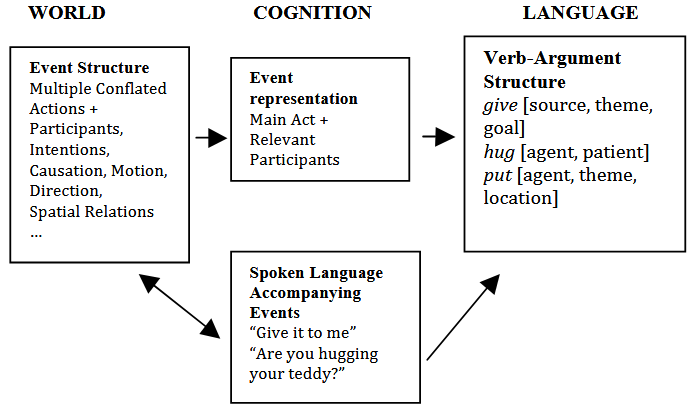
\includegraphics[width=0.50\colwidth]{figures/gordon2003_fig1.png}
      \caption{Mapping relations between events and language in the acquisition of verb-argument structure (Gordon, 2003).}
    \end{figure}

  \end{block}

  \begin{alertblock}{Prior Work: Gordon (2003)}

    Using a \textbf{habituation paradigm} with looped event videos:

    \begin{itemize}
      \item In GIVE vs.\ HUG, \textbf{10-month-olds} dishabituated when the toy was removed from GIVE but \textit{not} from HUG, suggesting the toy is relevant to GIVE's argument structure.
      \item \textbf{8-month-olds} showed a marginal GIVE effect ($p$=.07); \textbf{6-month-olds} showed no effect.
      \item In a separate SHOW experiment, even \textbf{10-month-olds} failed to dishabituate when the toy was removed, suggesting information transfer requires more advanced conceptualization.
    \end{itemize}

    \begin{figure}
      \centering
      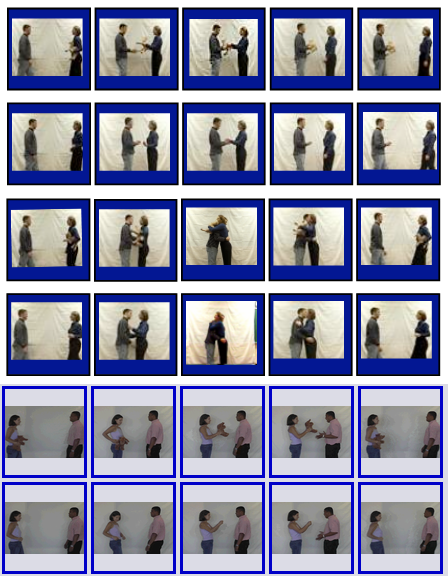
\includegraphics[width=0.48\colwidth]{figures/gordon2003_timelapse.png}
      \caption{Stimulus video frames. Rows 1-4: GIVE w/ toy, GIVE w/o, HUG w/ toy, HUG w/o. Rows 5-6: SHOW w/ toy, SHOW w/o (Gordon, 2003).}
    \end{figure}

    \begin{figure}
      \centering
      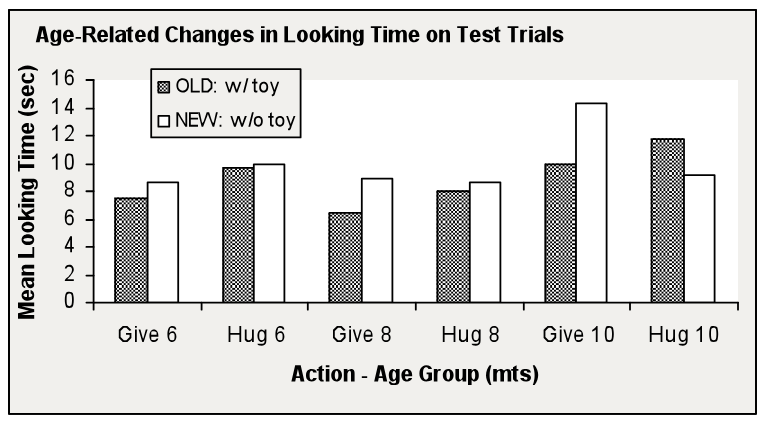
\includegraphics[width=0.52\colwidth]{figures/gordon2003_age_changes.png}
      \caption{Age-related changes in looking time on test trials for GIVE and HUG across 6, 8, and 10 months (Gordon, 2003).}
    \end{figure}

  \end{alertblock}

\end{column}

\separatorcolumn

% =====================================================================
% COLUMN 2: Methods & Results (GIVE)
% =====================================================================
\begin{column}{\colwidth}

  \begin{block}{Research Questions}

    \begin{enumerate}
      \item Do gaze transition patterns change from 7 to 11 months, specifically away from Toy$\leftrightarrow$Body transitions and toward Face$\leftrightarrow$Face transitions?
      \item Do GIVE and SHOW differ in the developmental trajectory of these gaze patterns?
    \end{enumerate}

  \end{block}

  \begin{block}{Methods}

    \heading{Participants}

    40 infants (7-11 months) and 15 adults in a within-subjects design. All participants viewed both GIVE and SHOW events; usable sample sizes varied by condition after data-quality screening (GIVE: $n$=40, SHOW: $n$=45).

    \heading{Stimuli \& EOI Coding}

    Participants viewed looped videos of GIVE and SHOW events. Rather than screen-based AOIs, we applied a custom computer-vision pipeline (\textbf{Eye-Track-ML}; Gushiken, Li, \& Gordon, 2025) to detect and segment event elements frame by frame, yielding dynamic \textbf{Elements of Interest (EOIs)}.

    \begin{figure}
      \begin{center}
      \begin{minipage}[c]{0.38\colwidth}
        \centering
        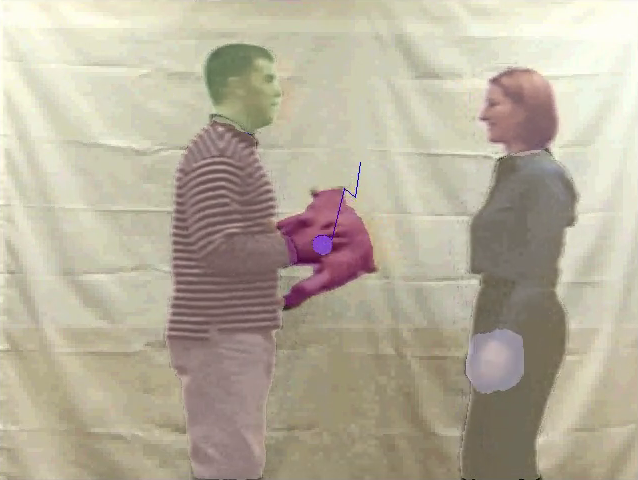
\includegraphics[width=\textwidth]{figures/eoi_stimulus.png}
      \end{minipage}%
      \hspace{0.04\colwidth}%
      \begin{minipage}[c]{0.15\colwidth}
        \centering
        
\includegraphics[width=0.75\textwidth]{figures/eyetrackml_qr.png}\\[0.5ex]
        {\scriptsize \textbf{Eye-Track-ML}\\Gushiken et al.,\\2025}
      \end{minipage}
      \end{center}
      \caption{GIVE stimulus frame with Eye-Track-ML SAM overlay showing segmented EOIs: body, head, and hand regions for each person, and the toy.}
    \end{figure}

    \heading{Statistical Approach}

    Gaussian GEE weighted by trial transition count, testing linear age trends (7-11 months). Fixation threshold: $\geq$3 consecutive frames; trial inclusion: $\geq$50\% on-screen looking.

  \end{block}

  \begin{block}{Results: GIVE Condition}

    \begin{figure}
      \centering
      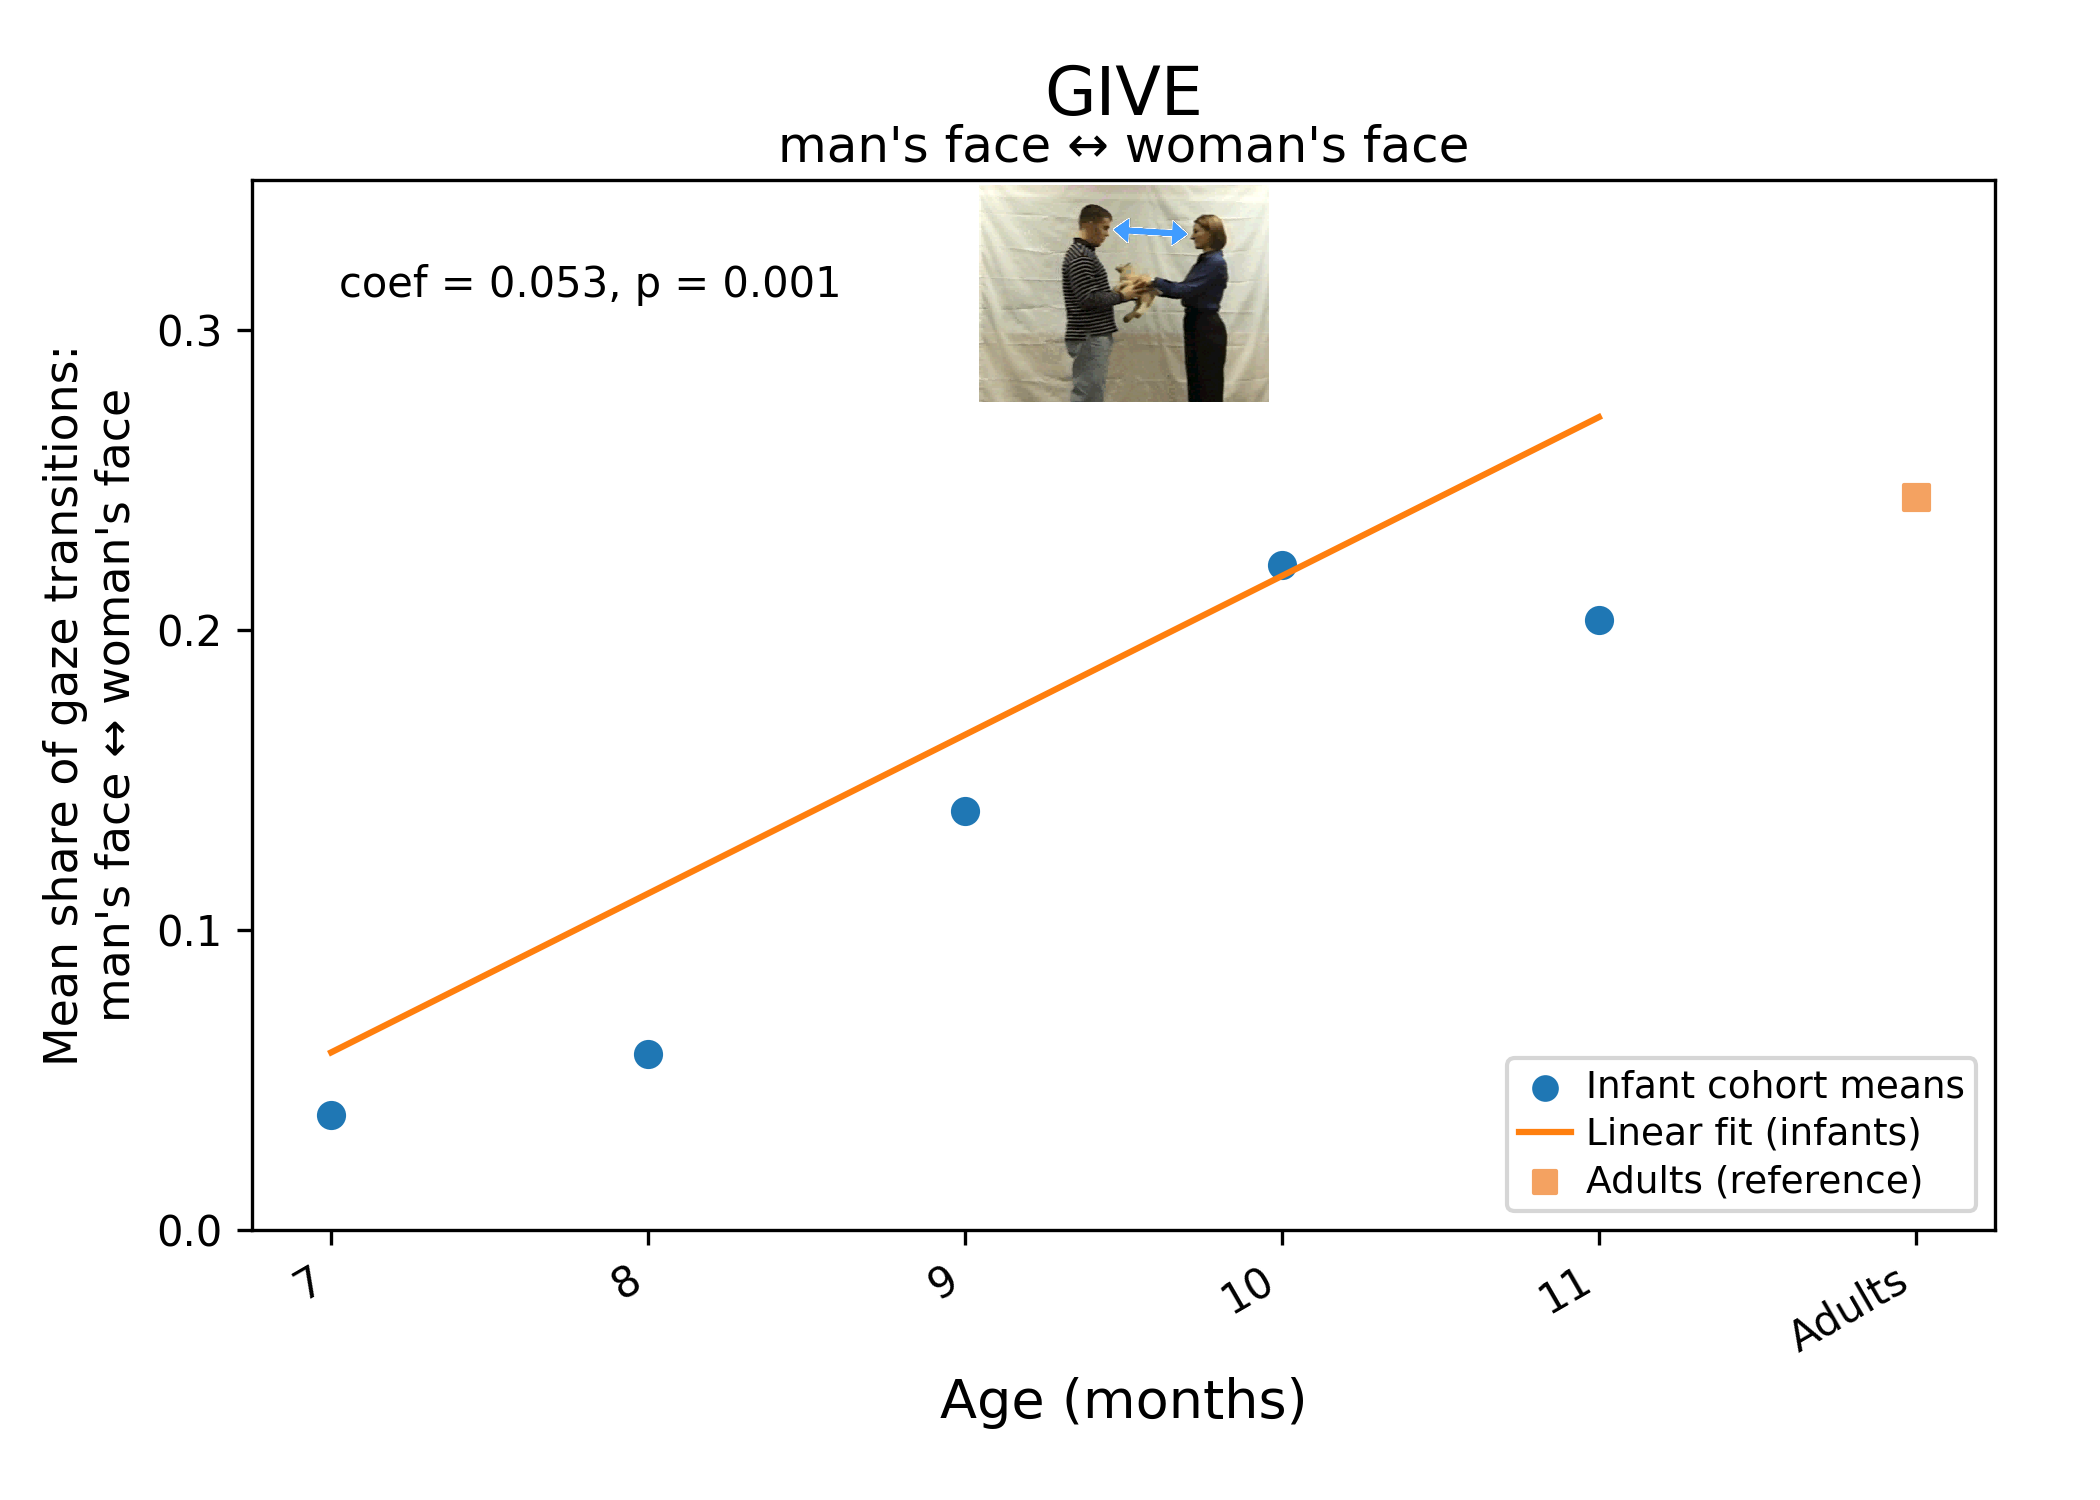
\includegraphics[width=0.52\colwidth]{figures/give_social_attention.png}
      \caption{GIVE: Face$\leftrightarrow$Face transitions increase significantly with age ($\beta$=0.053, $p$=.001). By 10-11 months, infants approached adult levels (20-22\% vs.\ 24.4\%).}
    \end{figure}

    \begin{figure}
      \centering
      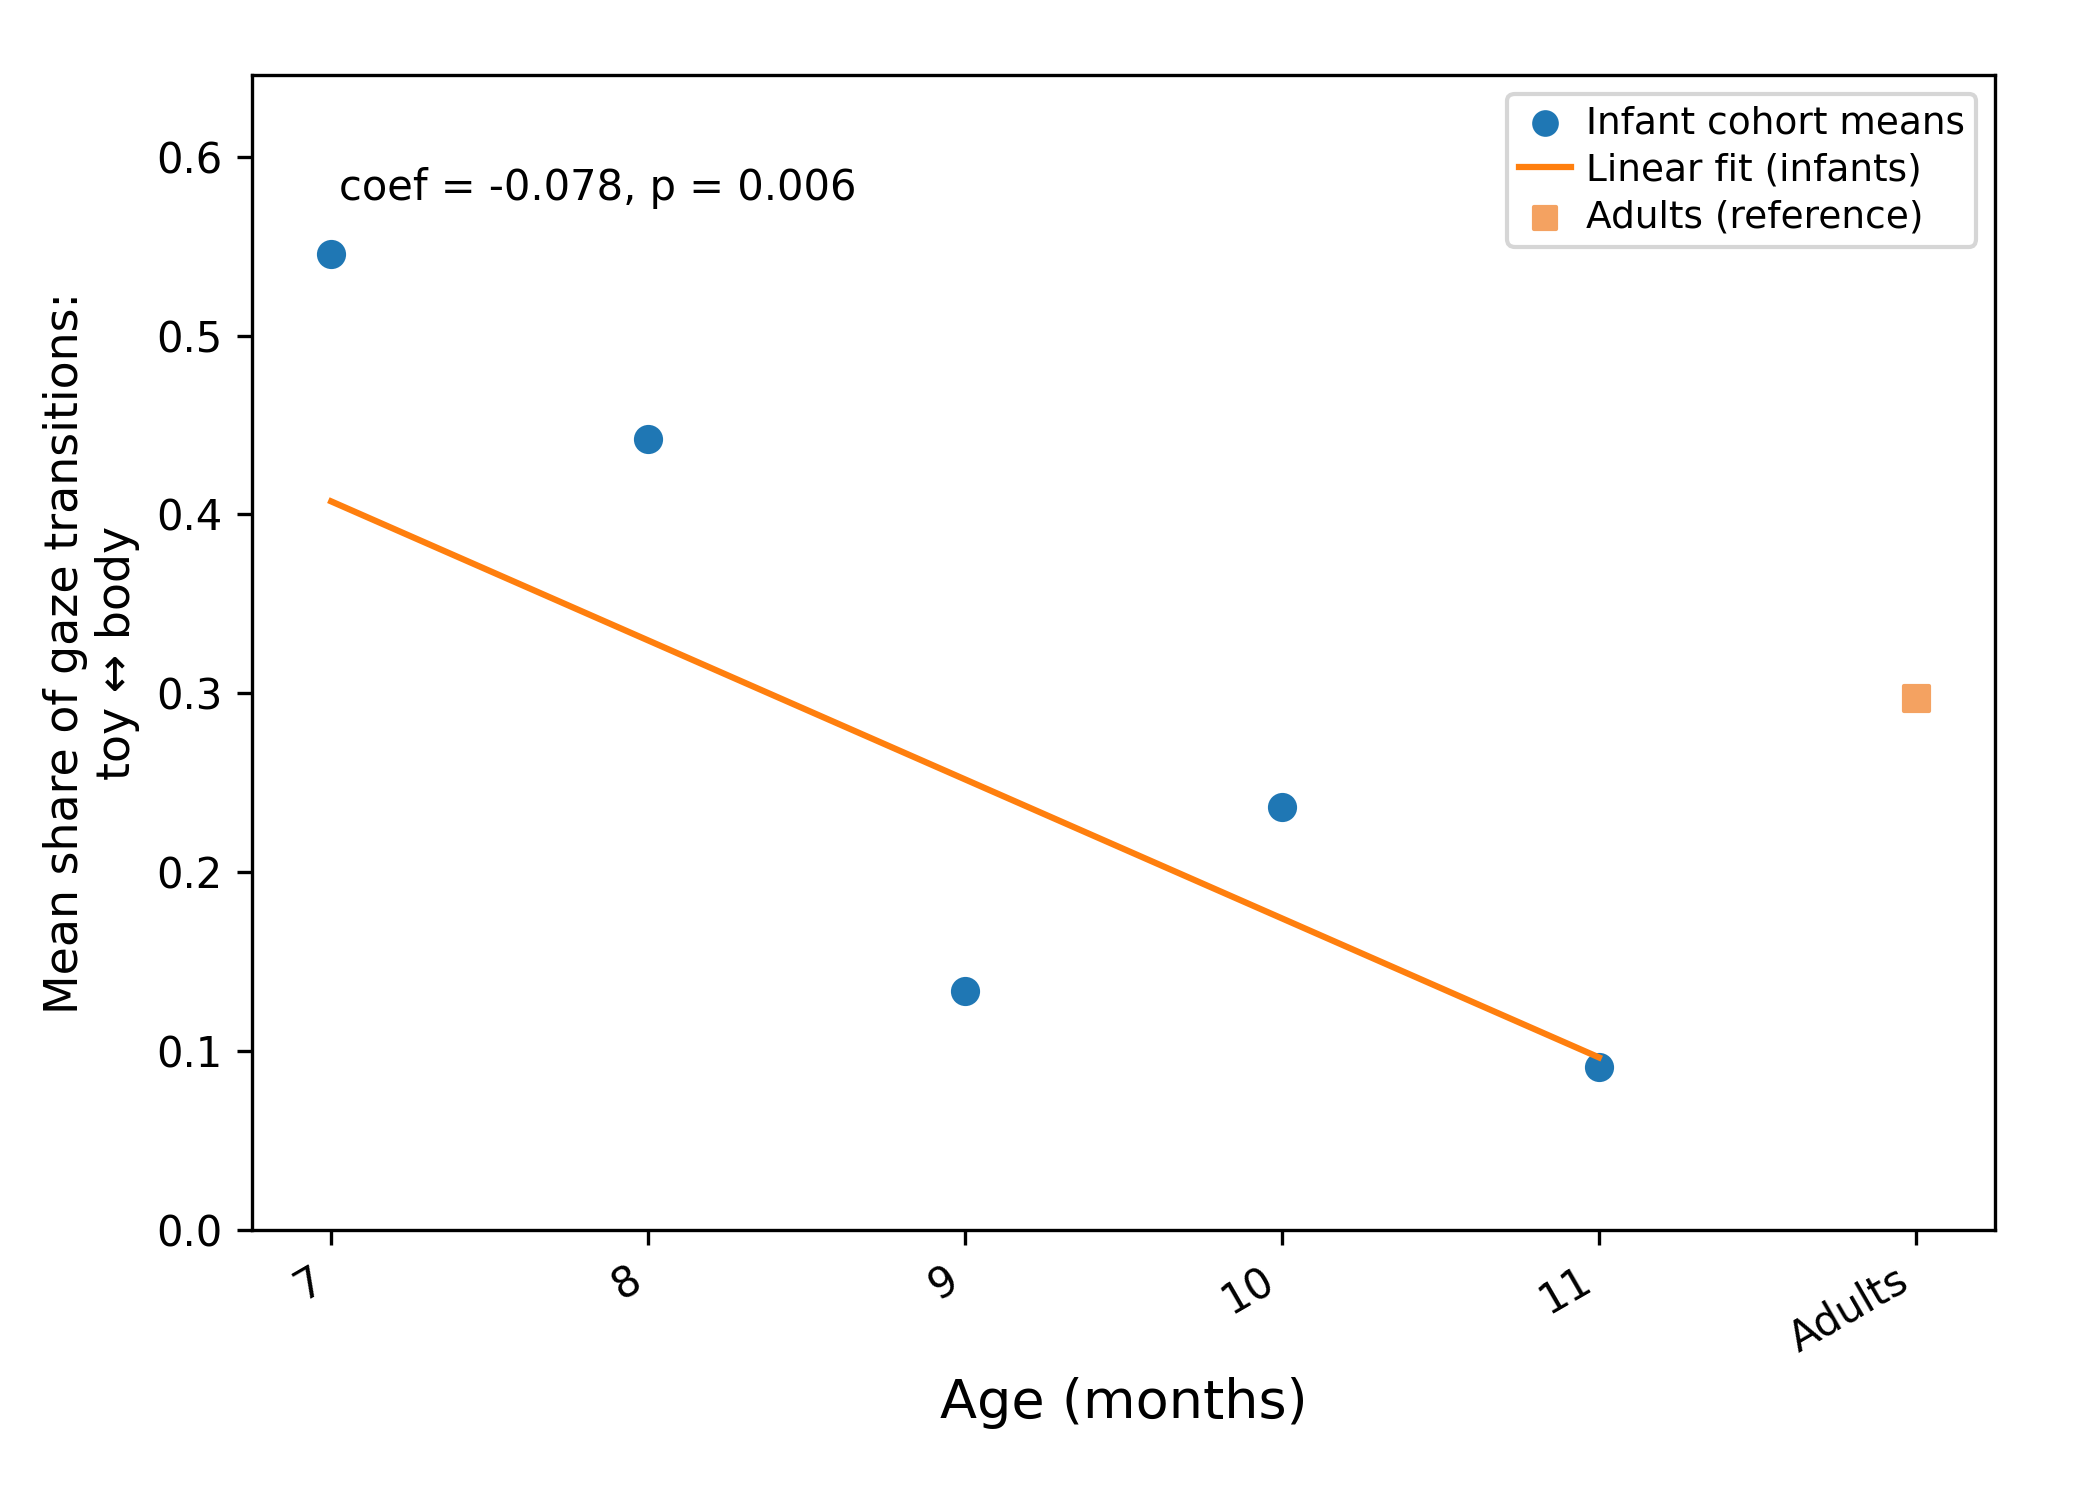
\includegraphics[width=0.52\colwidth]{figures/give_motion_tracking.png}
      \caption{GIVE: Toy$\leftrightarrow$Body transitions decrease significantly with age ($\beta$=$-$0.078, $p$=.006).}
    \end{figure}

  \end{block}

\end{column}

\separatorcolumn

% =====================================================================
% COLUMN 3: Results (SHOW), Comparison & Discussion
% =====================================================================
\begin{column}{\colwidth}

  \begin{block}{Results: SHOW Condition}

    \begin{figure}
      \centering
      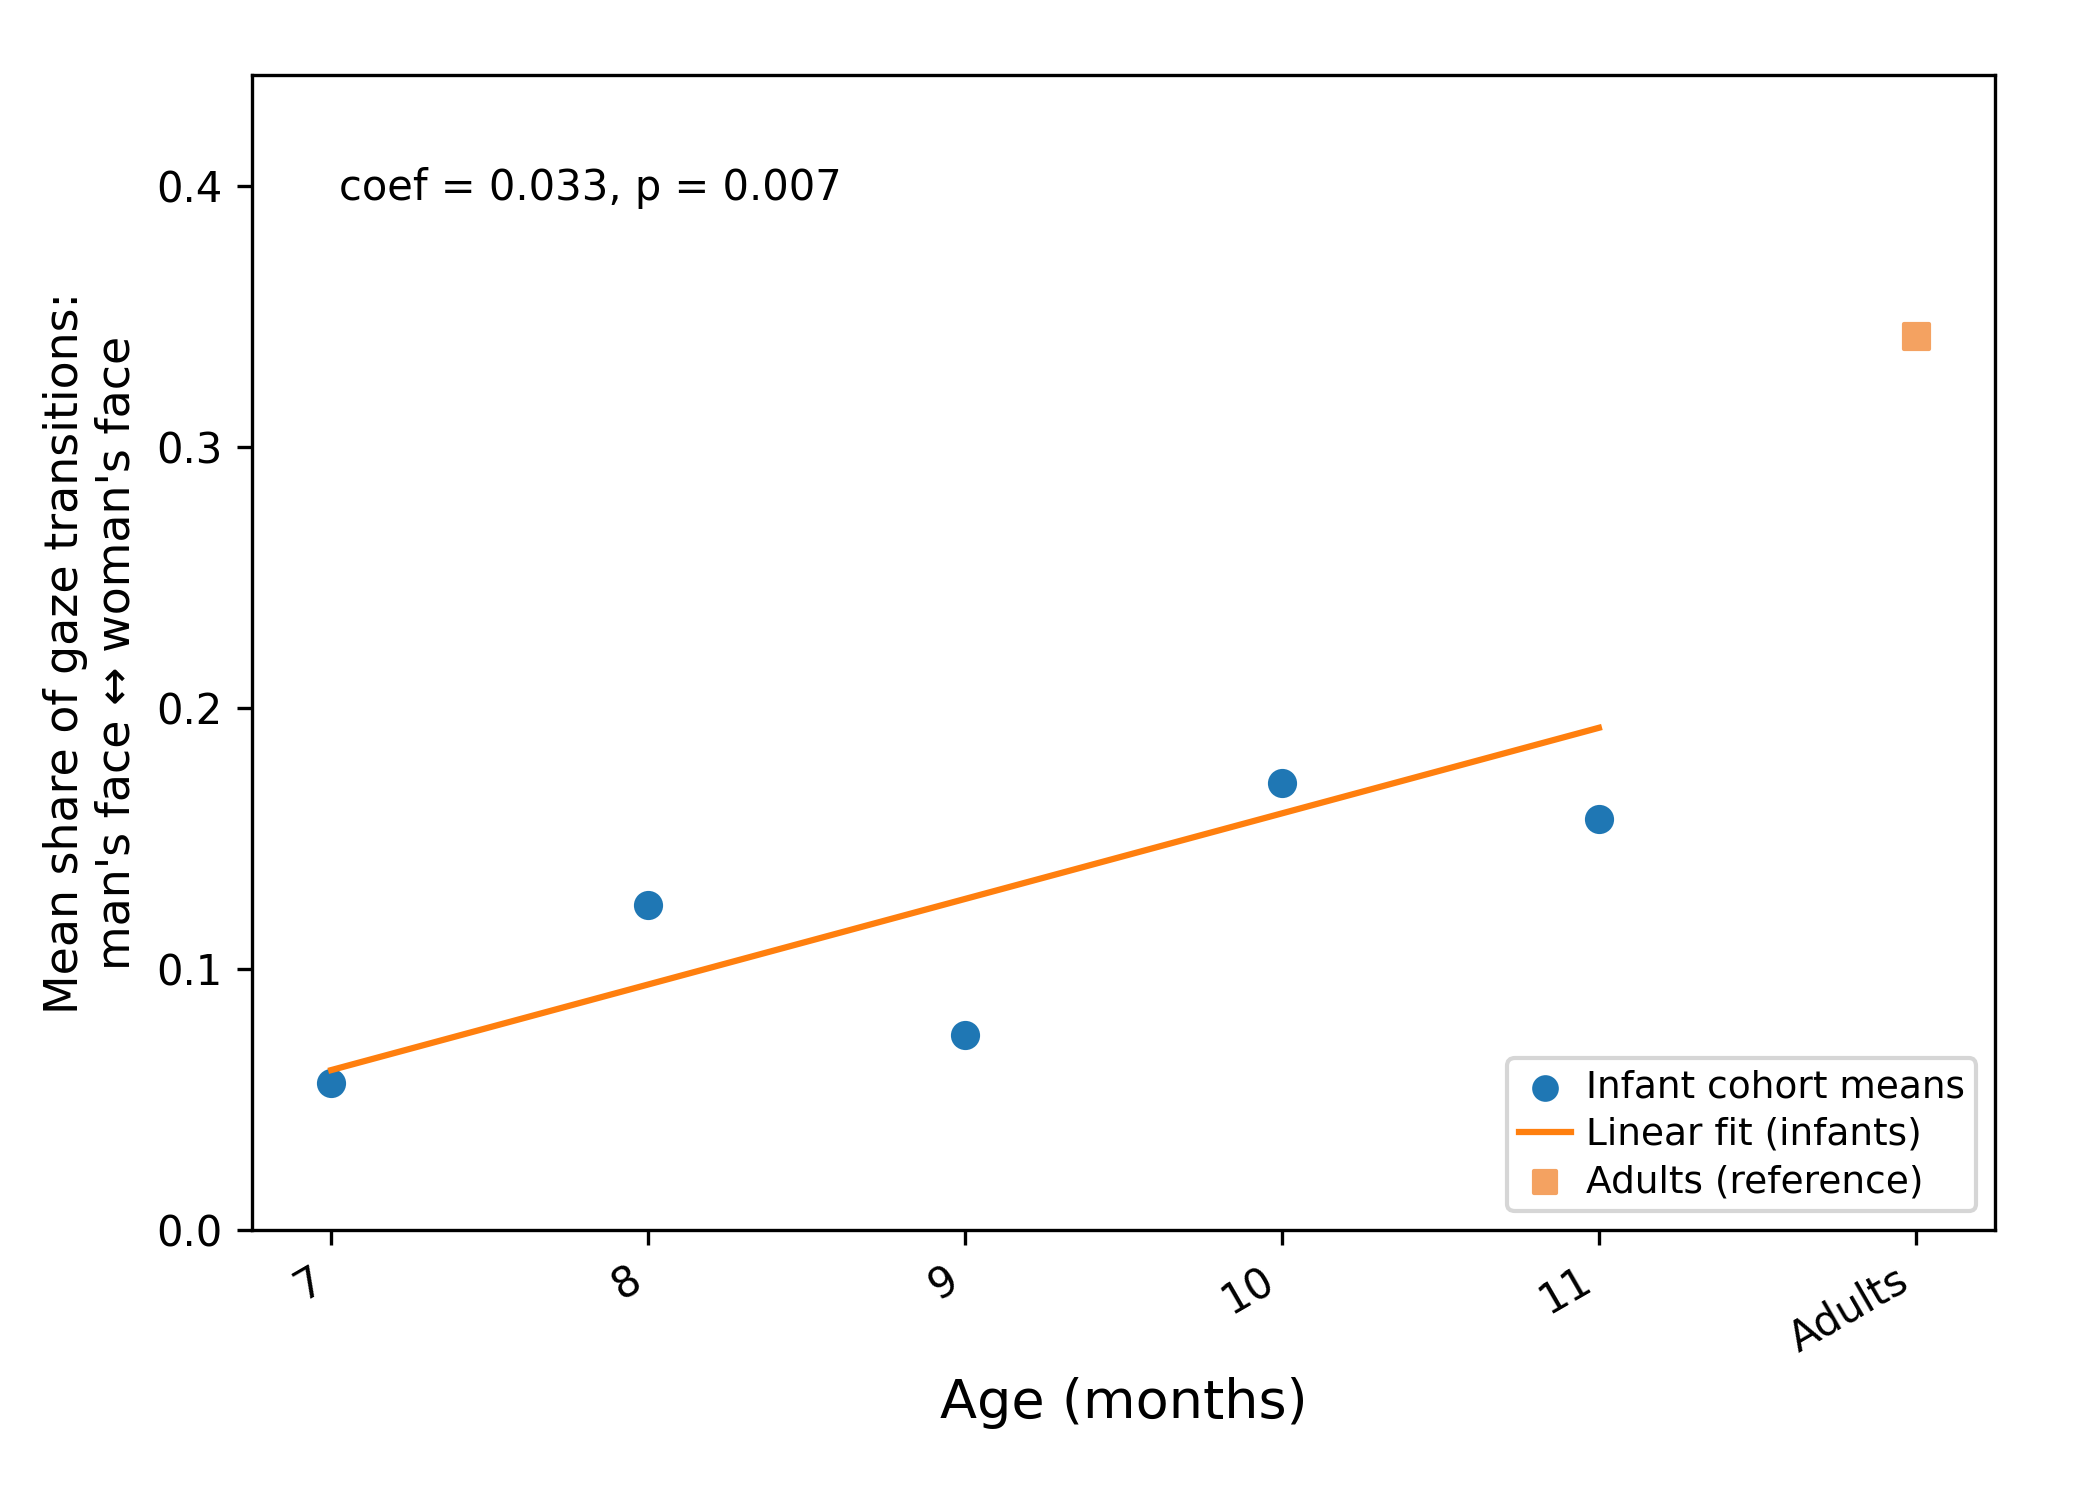
\includegraphics[width=0.52\colwidth]{figures/show_social_attention.png}
      \caption{SHOW: Face$\leftrightarrow$Face transitions increase with age ($\beta$=0.033, $p$=.007), but infants don't reach adult levels (15.8\% vs.\ 34.3\%).}
    \end{figure}

    \begin{figure}
      \centering
      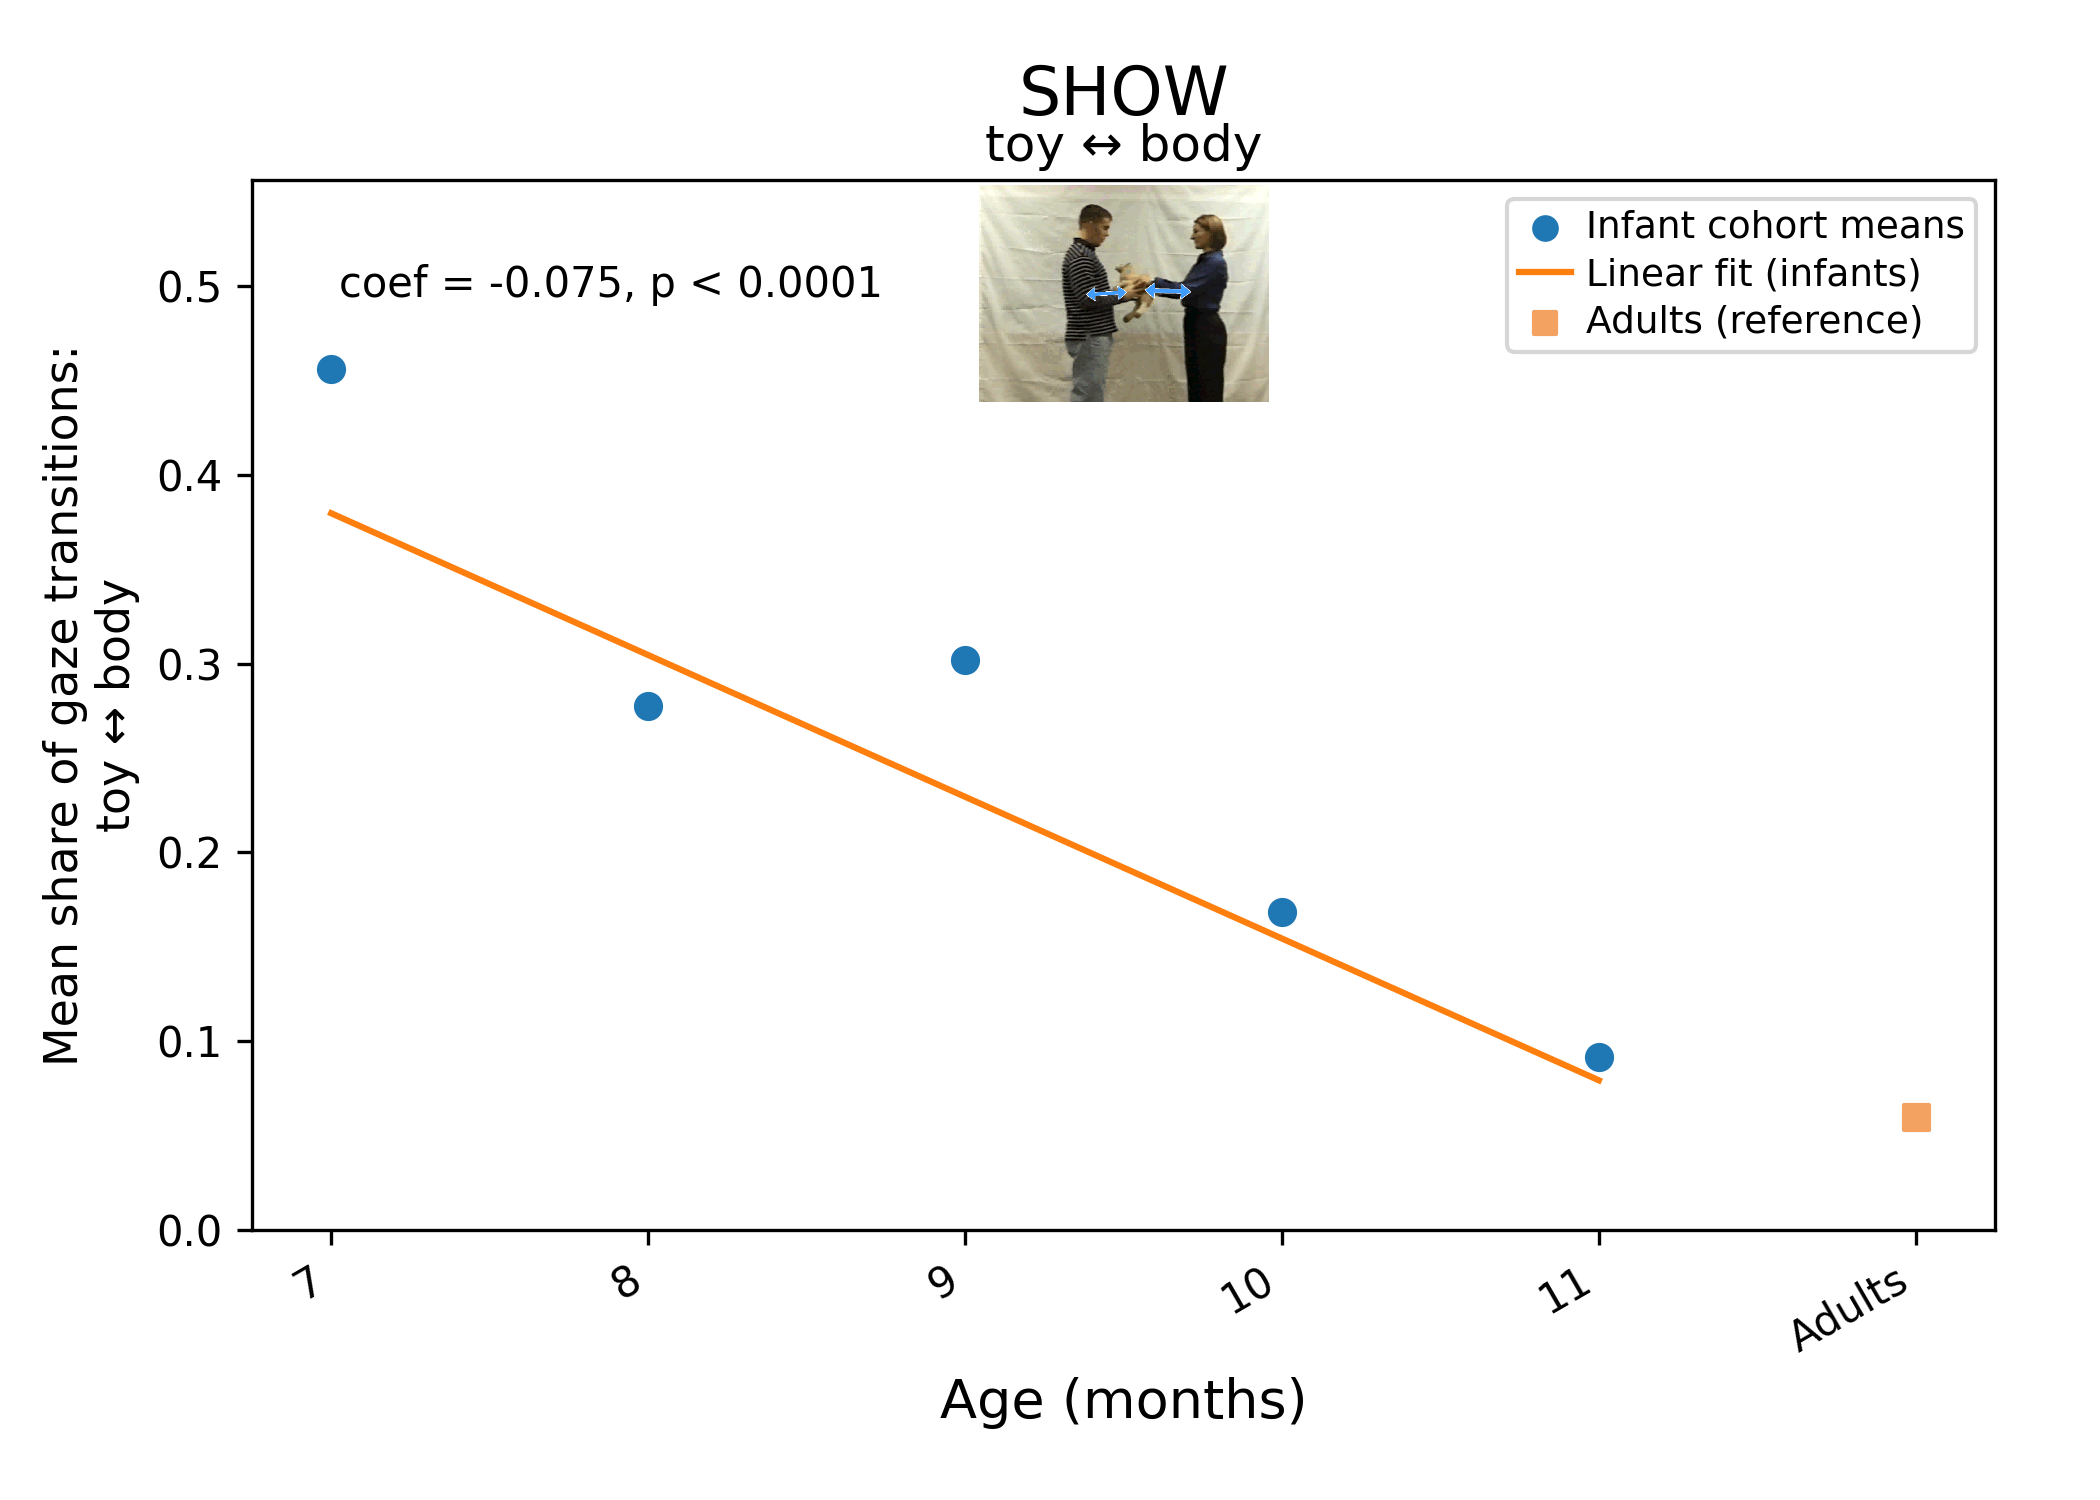
\includegraphics[width=0.52\colwidth]{figures/show_motion_tracking.png}
      \caption{SHOW: Toy$\leftrightarrow$Body transitions decrease with age ($\beta$=$-$0.075, $p$\textless .0001). By 11 months, infants approached adult levels (9.2\% vs.\ 6.0\%).}
    \end{figure}

  \end{block}

  \begin{alertblock}{GIVE vs.\ SHOW Comparison}

    \begin{table}
      \centering
      \begin{tabular}{l c c c}
        \toprule
        \textbf{Transition} & \textbf{Cond.} & $\boldsymbol{\beta}$ & \textbf{$p$} \\
        \midrule
        Face$\leftrightarrow$Face & GIVE & 0.053 & .001 \\
        Face$\leftrightarrow$Face & SHOW & 0.033 & .007 \\
        \midrule
        Toy$\leftrightarrow$Body & GIVE & $-$0.078 & .006 \\
        Toy$\leftrightarrow$Body & SHOW & $-$0.075 & \textless .0001 \\
        \midrule
        Toy$\leftrightarrow$Face & GIVE & 0.045 & .088 \\
        Toy$\leftrightarrow$Face & SHOW & 0.057 & \textless .0001 \\
        \bottomrule
      \end{tabular}
      \caption{Summary of linear age trends across GIVE and SHOW conditions.}
    \end{table}

    Infants approach adult-like gaze patterns for GIVE by 11 months but \textit{not} for SHOW, converging with Gordon (2003): GIVE event structure is parsed earlier than SHOW.

  \end{alertblock}

  \begin{block}{Take-Away}

    \textbf{Infants develop adult-like event parsing for GIVE by around 10-11 months but not for SHOW}, suggesting that \textit{physical transfer} is parsed before events requiring \textit{understanding of intention}. This converges with Gordon (2003), where infants dishabituated to toy removal in GIVE but not SHOW. The shift from Toy$\leftrightarrow$Body to Face$\leftrightarrow$Face transitions may reflect emerging understanding of \textbf{intentionality} and developing \textbf{theory of mind}, and may scaffold verb-argument structure acquisition.

  \end{block}

  \begin{block}{References}

    \footnotesize
    Gordon, P.\ (2003). The origin of argument structure in infant event representations. \textit{Unpublished manuscript.}\par
    Goldin-Meadow, S.\ (1985). Language development under atypical learning conditions. In K.\ Nelson (Ed.), \textit{Children's Language, Vol.\ 5.}\par
    Gushiken, M., Li, Y., \& Gordon, P.\ (2025). Eye-Track-ML. DOI:10.13140/RG.2.2.30558.34882\par
    Golinkoff, R.M.\ (1975). Semantic development in infants. \textit{Merrill-Palmer Quarterly, 21.}\par
    Baldwin, D.A.\ et al.\ (2001). Infants parse dynamic action. \textit{Child Development, 72.}\par
    Woodward, A.L.\ (1998). Infants selectively encode the goal object of an actor's reach. \textit{Cognition, 69.}

  \end{block}

\end{column}

\separatorcolumn
\end{columns}
\end{frame}

\end{document}
